\documentclass[12pt]{article}
\usepackage[paper=letterpaper,margin=2cm]{geometry}
\usepackage{amsmath,amssymb,amsfonts}
\usepackage{newtxtext,newtxmath}
\usepackage{enumitem}
\usepackage{titling}
\usepackage{subfig,graphicx}
\usepackage[colorlinks=true]{hyperref}
\usepackage{multirow}
\usepackage{listings}
\usepackage{xcolor}
\usepackage{float}

\definecolor{codegreen}{rgb}{0,0.6,0}
\definecolor{codegray}{rgb}{0.5,0.5,0.5}
\definecolor{codepurple}{rgb}{0.58,0,0.82}
\definecolor{backcolour}{rgb}{0.95,0.95,0.92}

\newcommand{\ind}{\perp\!\!\!\perp}

\lstdefinestyle{mystyle}{
    commentstyle=\color{codegreen},
    keywordstyle=\color{magenta},
    numberstyle=\tiny\color{codegray},
    stringstyle=\color{codepurple},
    basicstyle=\ttfamily\footnotesize,
    breakatwhitespace=false,
    breaklines=true,
    captionpos=b,
    keepspaces=true,
    numbers=left,
    numbersep=5pt,
    showspaces=false,
    showstringspaces=false,
    showtabs=false,
    tabsize=2
}
\lstset{style=mystyle}

\begin{document}

\begin{center}
\large{Aprendizagem 2023}\\
Homework II -- Group 28\\
\vskip 0.3cm
Gonçalo Bárias (ist1103124) \& Raquel Braunschweig (ist1102624)\vskip 1cm

\large{\textbf{Part I}: Pen and Paper}\normalsize
\end{center}

\noindent Consider the following dataset ($y_3$ - $y_5$ are all categorical variables and the domain of $y_2$ is $[0,1]$):

\begin{figure}[H]
    \centering
    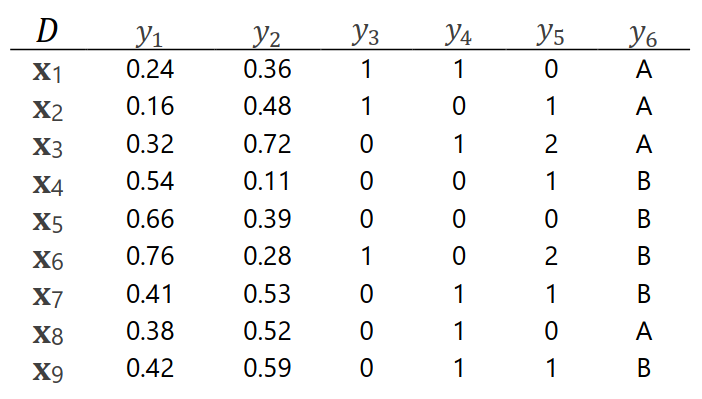
\includegraphics[width=9cm]{./assets/dataset_d.png}
    \label{fig:PartI-dataset-d}
\end{figure}

\begin{enumerate}[leftmargin=\labelsep]
    \item \textbf{Consider $x_1$ - $x_7$ to be training observations, $x_8$ - $x_9$ to be testing observations, $y_1$ - $y_5$ to be input
          variables and $y_6$ to be the target variable.\\
          \textit{Hint}: you can use \texttt{scipy.stats.multivariate\_normal} for multivariate distribution calculus}
          \begin{enumerate}
          \item \textbf{Learn a Bayesian classifier assuming: i) $\{y_1, y_2\}$, $\{y_3, y_4\}$ and $\{y_5\}$ sets of independent
                variables (e.g., $y_1 \ind y_3$ yet $y_1 \not\!\ind y_2$), and ii) $y_1 \times y_2 \in \mathbb{R}^{2}$ is normally distributed. Show all
                parameters (distributions and priors for subsequent testing).}

          \vskip 0.3cm
          Gonçalo

          \item \textbf{Under a MAP assumption, classify each testing observation showing all your calculus.}

          \vskip 0.3cm
          Gonçalo

          \item \textbf{Consider that the default decision threshold of $\theta = 0.5$ can be adjusted according to}

                \[
                        f(\textbf{x}|\theta)=
                    \begin{cases}
                        A,& P(A|\textbf{x}) > \theta\\
                        B,& \text{otherwise}
                    \end{cases}
                \]

                \textbf{Under a maximum likelihood assumption, what thresholds optimize testing accuracy?}

          \vskip 0.3cm
          Raquel
          \end{enumerate}

    \item \textbf{Let $y_1$ be the target numeric variable, $y_2$ - $y_6$ be the input variables where $y_2$ is binarized under an
          equal-width (equal-range) discretization. For the evaluation of regressors, consider a 3-fold
          cross-validation over the full dataset ($x_1$ - $x_9$) without shuffling the observations.}
          \begin{enumerate}
          \item \textbf{Identify the observations and features per data fold after the binarization procedure.}

          \vskip 0.3cm
          Raquel

    \item \textbf{Consider a distance-weighted kNN with k = 3, Hamming distance (\textit{d}), and 1 / \textit{d} weighting.
          Compute the MAE of this kNN regressor for the $1^{st}$ iteration of the cross-validation (i.e. train
          observations have the lower indices).}

          \vskip 0.3cm
          Raquel
          \end{enumerate}
\end{enumerate}

\vskip 0.5cm

\begin{center}
\large{\textbf{Part II}: Programming and critical analysis}\normalsize
\end{center}

\noindent Considering the \texttt{column\_diagnosis.arff} dataset available at the course webpage’s homework tab. Using \texttt{sklearn}, apply a 10-fold stratified
cross-validation with shuffling (\texttt{random\_state=0}) for the assessment of predictive models along this section.

\begin{enumerate}[leftmargin=\labelsep]
    \item \textbf{Compare the performance of kNN with k = 5 and Naïve Bayes with Gaussian assumption
          (consider all remaining parameters for each classifier as \texttt{sklearn}'s default):}
          \begin{enumerate}
          \item \textbf{Plot two boxplots with the fold accuracies for each classifier.}

          \vskip 0.3cm
          \lstinputlisting[language=Python]{./assets/code_1a.py}

          \begin{figure}[H]
            \centering
            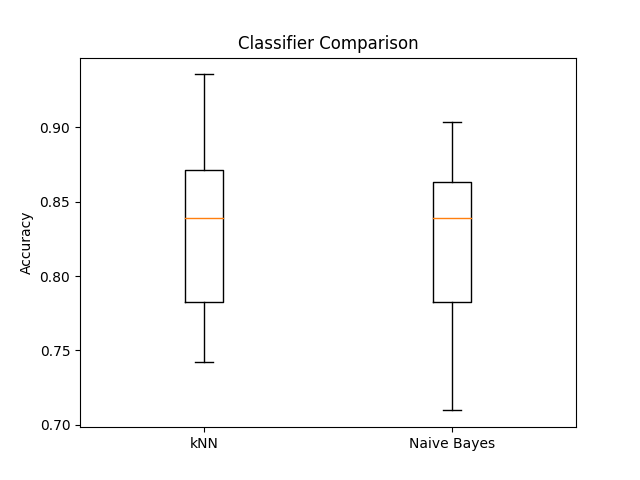
\includegraphics[width=13cm]{./assets/II-1-graph.png}
            \caption{10-Fold Cross-Validation Results for kNN and Naive Bayes on Column Diagnosis Dataset}
            \label{fig:PartII-ex1}
        \end{figure}

          \item \textbf{Using \texttt{scipy}, test the hypothesis "kNN is statistically superior to Naïve Bayes regarding
                accuracy", asserting whether is true.}

          \vskip 0.3cm
          \lstinputlisting[language=Python]{./assets/code_1b.py}

          \textbf{Answer:} Fail to reject null hypothesis: No significant difference in accuracy between kNN and Naive Bayes
          \end{enumerate}

    \item \textbf{Consider two kNN predictors with k = 1 and k = 5 (uniform weights, Euclidean distance,
          all remaining parameters as default). Plot the differences between the two cumulative confusion
          matrices of the predictors. Comment.}

          \vskip 0.3cm
          \lstinputlisting[language=Python]{./assets/code_2.py}

          \begin{figure}[H]
              \centering
              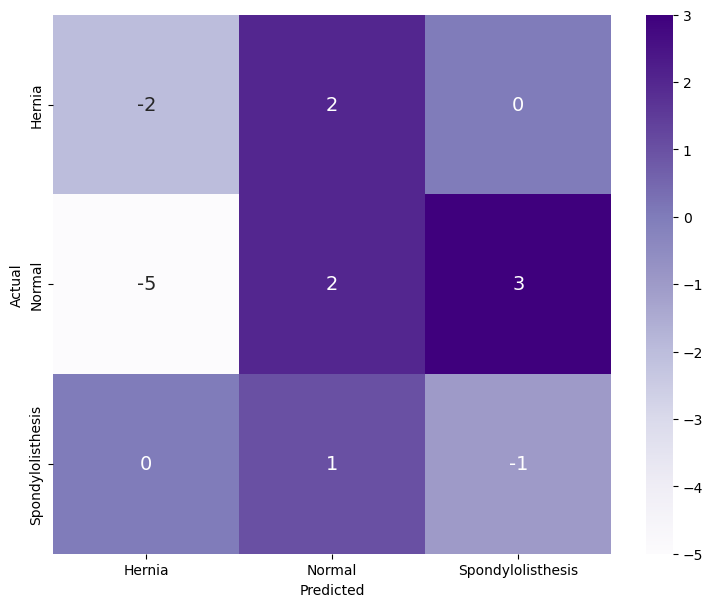
\includegraphics[width=13cm]{./assets/cummulative_heatmap_ex2_PartII.png}
              \caption{Confusion Matrix Differences Between k=1 and k=5 k-Nearest Neighbors (kNN) Classifiers}
              \label{fig:PartII-ex2}
          \end{figure}

          Blah % TODO: Need to comment the plot

    \item \textbf{Considering the unique properties of \texttt{column\_diagnosis}, identify three possible difficulties
          of naïve Bayes when learning from the given dataset.}

          \vskip 0.3cm
          Gonçalo
\end{enumerate}

\end{document}
